\documentclass[10pt]{article}
\usepackage{../pplmanual}

\newcommand{\function}[1]{{\noindent{\textsf{#1}}\\}}
\newcommand{\args}[1]{\hspace*{2em}{\texttt{#1}}\\}
\newcommand{\param}[1]{{\texttt{#1}}}
\newcommand{\kw}[1]{{\textsf{#1}}}
\newcommand{\uw}[1]{{\textsl{#1}}}

\makeindex

\title{Charm++\\ Finite Element Framework\\ Manual}
\version{1.0}
\credits{
Initial version of Charm++ Finite Element Framework was developed
by Milind Bhandarkar with inputs from Timothy Hinrichs and Kathikeyan
Mahesh. The current version is almost completely rewritten by
Orion Lawlor.
}

\begin{document}

\maketitle

\section{Motivation}

The Finite Element Method (FEM) approach is used in many engineering
applications with irregular domains, from elastic deformation problems to
crack propagation to fluid flow.  Charm++ is a free message-passing parallel
runtime system for machines from clusters of workstations to tightly-coupled
SMPs.  The Charm++ FEM framework allows you to write a parallel FEM program,
in C or Fortran 90, with minor additional effort over the serial version.
Using the FEM framework also allows you to take advantage of all the
features of Charm++, including run-time load balancing,  performance
monitoring and visualization, and checkpoint/restart, with no additional
effort.


\section{Introduction/Terminology}

A FEM program manipulates elements and nodes. An element is a portion of
the problem domain, typically in the shape of a triangle, square, or hexagon
in 2D; or tetrahedron or rectangular solid in 3D.  A node is a point in the
domain.  An element knows which nodes surround it via the connectivity
table, which lists adjacent nodes.

\begin{figure}[h]
\begin{center}
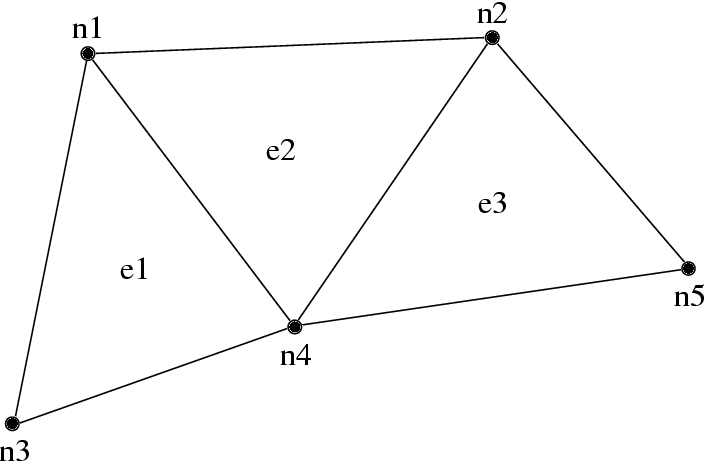
\includegraphics[width=4in]{simple_mesh}
\end{center}
\caption{3-element, 5 node mesh.}
\label{fig:simplemesh}
\end{figure}

\begin{table}[h]
\begin{center}
\begin{tabular}{||l||r|r|r||}\hline
Element & \multicolumn{3}{c||}{Adjacent Nodes} \\\hline
e1 & n1 & n3 & n4 \\
e2 & n1 & n2 & n4 \\
e3 & n2 & n4 & n5 \\
\hline
\end{tabular}
\end{center}
\caption{Connectivity table for mesh in figure~\ref{fig:simplemesh}.}
\label{table:simplemesh}
\end{table}

A typical FEM program performs some element-by-element calculations which
update adjacent node values; then some node-by-node calculations.  For
example, a material dynamics program has the structure:

\begin{alltt}
     time loop
          element loop-- Element deformation applies forces to
          surrounding nodes
          node loop-- Forces and boundary conditions change node
          positions
     end time loop
\end{alltt}

We can parallelize such FEM programs by partitioning the serial mesh
elements into several chunks  (at least one chunk per processor; perhaps
even more).  During partitioning, we give nodes and elements new,
chunk-local numbers.  Below, we partition the mesh above into two chunks, A
and B.

\begin{figure}[h]
\begin{center}
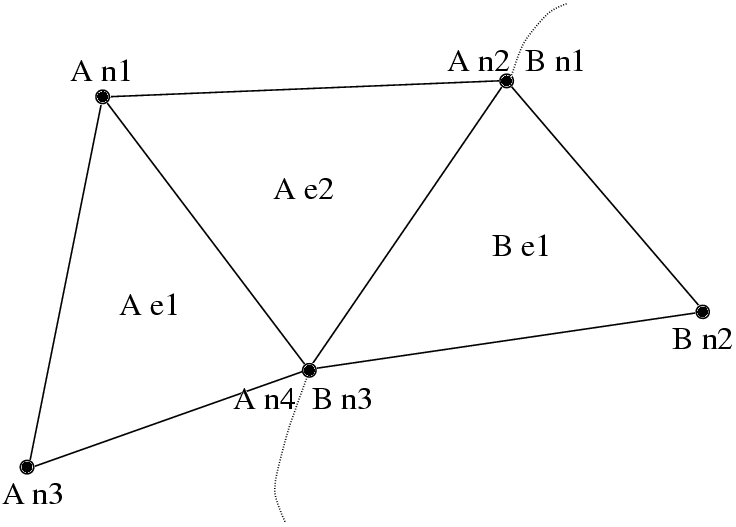
\includegraphics[width=4in]{partitioned_mesh}
\end{center}
\caption{Partitioned mesh.}
\label{fig:partitionedmesh}
\end{figure}

\begin{table}[h]
\begin{center}
\begin{tabular}{||l||r|r|r||}\hline
Element & \multicolumn{3}{c||}{Adjacent Nodes} \\\hline
e1 & n1 & n3 & n4 \\
e2 & n1 & n2 & n4 \\
\hline
\end{tabular}
\end{center}
\caption{Connectivity table for chunk A in figure~\ref{fig:partitionedmesh}.}
\label{table:chunkA}
\end{table}

\begin{table}[h]
\begin{center}
\begin{tabular}{||l||r|r|r||}\hline
Element & \multicolumn{3}{c||}{Adjacent Nodes}\\\hline
e1 & n1 & n2 & n3 \\
\hline
\end{tabular}
\end{center}
\caption{Connectivity table for chunk B in figure~\ref{fig:partitionedmesh}.}
\label{table:chunkB}
\end{table}

Note that chunk A's node n2 and B's node n1 were actually the same node in
the original mesh-- partitioning split this single node into two shared
copies (one on each chunk).  However, since adding forces is associative, we
can handle shared nodes by computing the forces normally (ignoring the
existence of the other chunk), then adding both chunks' net force for the
shared node together.  This ``node update'' will give us the same resulting
force on each shared node as we would get without partitioning, thus the
same positions, thus the same final result.  Hence, each chunk's time loop
has the structure:

\begin{alltt}
     chunk time loop
          element loop-- Element deformation applies forces to
          surrounding nodes
          <update forces on shared nodes>
          node loop-- Forces and boundary conditions change node
          positions
     end time loop
\end{alltt}

This is exactly the form of the time loop for a Charm++ FEM framework
program.  The framework will accept a serial mesh, partition it, distribute
the chunks to each processor, allow the user to run their time loop, and
handle the node-updates.


\section{Structure of a FEM Framework Program}

A FEM framework program consists of three subroutines: \kw{init}, \kw{driver},
and \kw{finalize}.  \kw{init} and \kw{finalize} are called by the FEM framework
only on the first processor -- these routines typically do specialized I/O,
startup and shutdown tasks.  \kw{driver} is called for every chunk on every
processor, and does the main work of the program.

\begin{alltt}
     subroutine init
          read the serial mesh and configuration data
     end subroutine

     subroutine driver
          get local mesh chunk
          time loop
               FEM computations
               update shared node fields
               more FEM computations
          end time loop
     end subroutine

     subroutine mesh_updated
          write intermediate results; modify serial mesh
     end subroutine
     subroutine finalize
           write results
     end subroutine
\end{alltt}

\section{Compilation and Execution}

A FEM framework program is a Charm++ program, so you must begin by
downloading the latest source version of Charm++ from
{\tt http://charm.cs.uiuc.edu/}.  Build the source with 
{\tt ./SUPER\_INSTALL FEM version} or {\tt cd} into the build directory, 
{\tt version/tmp}, and type {\tt make FEM}.
To compile a FEM program, pass the {\tt -language fem} (for C) or 
{\tt -language femf} (for Fortran) option to {\tt charmc}.


\section{FEM Framework API Reference}

\subsection{Utility}

\function{int FEM\_Num\_Partitions();}
\function{function integer :: FEM\_Num\_Partitions()}

     Return the number of mesh chunks in the current computation.  Can
     only be called from the driver routine.

\function{int FEM\_My\_Partition();}
\function{function integer :: FEM\_My\_Partition()}

     Return the number of the current chunk, from 0 to
     \kw{num\_partitions}-1.  Can only be called from the driver routine.

\function{double FEM\_Timer();}
\function{function double precision :: FEM\_Timer()}

     Return the current wall clock time, in seconds.  Resolution is
     machine-dependent, but is at worst 10ms.

\function{void FEM\_Print\_Partition();}
\function{subroutine FEM\_Print\_Partition()}

     Print a debugging representation of the current chunk's mesh.
     Prints the entire connectivity array, and data associated with
     each local node and element.

\function{void FEM\_Print(const char *str);}
\function{subroutine FEM\_Print(str)}
\args{  character*, intent(in) :: str}

     Print the given string.  Works on all machines; unlike \kw{printf} or
     \kw{print *}, which may not work on all parallel machines.

\subsection{Mesh}

These routines describe and retreive the finite element mesh for this
computation.  A mesh, from the framework's perspective, is a list of
elements, nodes, uninterpreted data associated with each, and the
connectivity table.  Elements and nodes have both a global number (number in
the serial mesh) as well as a chunk-local number (number in the partitioned
mesh chunk).  The FEM framework currently uses the free Metis package for
partitioning.

A simple program would set the serial mesh in init, get the partitioned
chunk in driver, and work on that chunk.  A more complex program would set
the initial mesh in init; get, work on, update and repartition the mesh
several times in driver; and perform post-processing on the reassembled,
modified mesh in finalize.

From \kw{init()}, the \kw{FEM\_Set\_} routines describe the serial mesh, which
will be partitioned into chunks.

From \kw{driver()}, the \kw{FEM\_Get\_} routines ask for the current mesh
chunk; the \kw{FEM\_Set\_} routines describe a new partitioned mesh chunk.  The
new chunk need not have the same number of elements or nodes as the old chunk;
but any new added nodes are assumed private (not shared).
\kw{FEM\_Update\_Mesh} will reassemble a serial version of the mesh from the
new pieces and optionally repartition the serial mesh.

From \kw{mesh\_updated()}, the \kw{FEM\_Get} and \kw{FEM\_Set} routines
manipulate the serial mesh.   \kw{Mesh\_updated} is only executed if you call
\kw{FEM\_Update\_Mesh} during driver-- otherwise, \kw{mesh\_updated} can be an
empty procedure.  The parameter \kw{callMeshUpdated} is passed down to
\kw{mesh\_update}.

From \kw{finalize(),} the \kw{FEM\_Get\_} routines ask for the reassembled
serial mesh-- for this, you must have previously called \kw{FEM\_Update\_Mesh}
during driver.

\function{void FEM\_Set\_Mesh(int nElem, int nNodes, int nodePerEl,const int* conn);}

     This is a convenience routine equivalent to:
\begin{alltt}
          FEM\_Set\_Node(nNodes,0);
          FEM\_Set\_Elem(0,nElem,0,nodePerEl);
          FEM\_Set\_Elem\_Conn(0,conn);
\end{alltt}

\function{subroutine FEM\_Set\_Mesh(nElem,nNodes,nodePerEl,conn)}
    \args{integer, intent(in) :: nElem, nNodes, nodePerEl}
    \args{integer, intent(in), dimention(nElem,nodePerEl) :: conn;}

     This is a convenience routine equivalent to:
\begin{alltt}
          CALL FEM\_Set\_Node(nNodes,0)
          CALL FEM\_Set\_Elem(1,nElem,0,nodePerEl)
          CALL FEM\_Set\_Elem\_Conn\_c(1,conn)
\end{alltt}

\function{void FEM\_Set\_Elem(int elType,int  nEl,int  doublePerEl,int  nodePerEl);}
\function{void FEM\_Get\_Elem(int elType,int *nEl,int *doublePerEl,int *nodePerEl);}
\function{subroutine FEM\_Set\_Elem(elType,nEl,doublePerEl,nodePerEl)}
  \args{integer, intent(in)  :: elType,nEl,doublePerEl,nodePerEl}
\function{subroutine FEM\_Get\_Elem(elType,nEl,doublePerEl,nodePerEl)}
  \args{integer, intent(in)  :: elType}
  \args{integer, intent(out) :: nEl,doublePerEl,nodePerEl}

     Describe/retreive the number and type of elements.  \kw{ElType} is the
number of element types registered so far (the first element type is 1, then 2,
etc.).  \kw{nEl} is the number of elements being registered.  \kw{doublesPerEl}
and \kw{nodePerEl} are the number of doubles of user data, and nodes
(respectively) associated with each element.

     \kw{doublePerEl} or \kw{nodePerEl} may be zero, indicating that no user
data or connectivity data (respectively) is associated with the element.

\function{void FEM\_Set\_Elem\_Conn(int elType,const int *conn);}
\function{void FEM\_Get\_Elem\_Conn(int elType,int *conn);}
\function{subroutine FEM\_Set\_Elem\_Conn\_r(elType,conn)}
  \args{integer, intent(in)  :: elType}
  \args{integer, intent(in),  dimention(nodePerEl,nEl) :: conn}
\function{subroutine FEM\_Get\_Elem\_Conn\_r(elType,conn)}
  \args{integer, intent(in)  :: elType}
  \args{integer, intent(out), dimention(nodePerEl,nEl) :: conn}
\function{subroutine FEM\_Set\_Elem\_Conn\_c(elType,conn)}
  \args{integer, intent(in)  :: elType}
  \args{integer, intent(in),  dimention(nEl,nodePerEl) :: conn}
\function{subroutine FEM\_Get\_Elem\_Conn\_c(elType,conn)}
  \args{integer, intent(in)  :: elType}
  \args{integer, intent(out), dimention(nEl,nodePerEl) :: conn}

     Describe/retreive the element connectivity array for this element
     type.  The connectivity array is indexed by the element number,
     and gives the indices of the nodes surrounding the element.  It is
     hence \kw{nodePerEl*nEl} integers long.

     The C version array indices are zero-based, and must be stored in
     row-major order (a given element's surrounding nodes are stored
     contiguously in the conn array).  The Fortran version indices are
     one-based, and are available in row-major (named \_r) and
     column-major (named \_c) versions.  We recommend row-major storage
     because it results in better cache utilization (because the nodes
     around an element are stored contiguously).

\function{void FEM\_Set\_Node(int  nNode,int  doublePerNode);}
\function{void FEM\_Get\_Node(int *nNode,int *doublePerNode);}
\function{subroutine FEM\_Set\_Node(nNode,doublePerNode)}
  \args{integer, intent(in)  :: nNode,doublePerNode}
\function{subroutine FEM\_Get\_Node(nNode,doublePerNode)}
  \args{integer, intent(out) :: nNode,doublePerNode}

     Describe/retreive the number of nodes and doubles of user data
     associated with each node.  There is only one type of node, so no
     \kw{nodeType} identifier is needed.

     \kw{doublePerNode} may be zero, indicating that no user data is
     associated with each node.

\function{void FEM\_Set\_Node\_Data(const double *data);}
\function{void FEM\_Get\_Node\_Data(double *data);}
\function{void FEM\_Set\_Elem\_Data(int elType,const double *data);}
\function{void FEM\_Get\_Elem\_Data(int elType,double *data);}
\function{subroutine FEM\_Set\_Node\_Data\_r(data)}
  \args{REAL*8, intent(in),  dimention(doublePerNode,nNode)  :: data}
\function{subroutine FEM\_Get\_Node\_Data\_r(data)}
  \args{REAL*8, intent(out), dimention(doublePerNode,nNode)  :: data}
\function{subroutine FEM\_Set\_Elem\_Data\_r(data)}
  \args{REAL*8, intent(in),  dimention(doublePerElem,nElem)  :: data}
\function{subroutine FEM\_Get\_Elem\_Data\_r(data)}
  \args{REAL*8, intent(out), dimention(doublePerElem,nElem)  :: data}
\function{subroutine FEM\_Set\_Node\_Data\_c(data)}
  \args{REAL*8, intent(in),  dimention(nNode,doublePerNode)  :: data}
\function{subroutine FEM\_Get\_Node\_Data\_c(data)}
  \args{REAL*8, intent(out), dimention(nNode,doublePerNode)  :: data}
\function{subroutine FEM\_Set\_Elem\_Data\_c(data)}
  \args{REAL*8, intent(in),  dimention(nElem,doublePerElem)  :: data}
\function{subroutine FEM\_Get\_Elem\_Data\_c(data)}
  \args{REAL*8, intent(out), dimention(nElem,doublePerElem)  :: data}

     Describe/retrieve the optional, uninterpreted user data associated with
each node and element.  This user data is partitioned and reassembled along
with the connectivity matrix, and may include initial conditions, boundary
values, or any other data needed or produced by the program.   The Fortran
arrays can be row- or column- major (see \kw{FEM\_Set\_Elem\_Conn} for
details).  The row-major form is preferred.

\function{void FEM\_Update\_Mesh(int callMeshUpdated,int doRepartition);}
\function{subroutine FEM\_Update\_Mesh(callMeshUpdated,doRepartition)}
    \args{integer, intent(in) :: callMeshUpdated,doRepartition}

     Reassemble the mesh chunks from each partition into a single serial mesh.
Can only be called from driver; and must be called by the driver routine for
every chunk.  The call is blocking only if \kw{doRepartition} is true;
otherwise the call will immediately return.  \kw{FEM\_Get} calls from
\kw{driver()} will only return the new mesh after a \kw{FEM\_Update\_Mesh} call
where \kw{doRepartition} is true; otherwise \kw{FEM\_Get} returns the old mesh.

     If \kw{callMeshUpdated} is not zero, \kw{mesh\_updated(callMeshUpdated)}
will be called on the first processor after the mesh is reassembled.

     If \kw{doRepartition} is 1, the reassembled serial mesh will be
repartitioned back into chunks and redistributed.  Otherwise,
\kw{FEM\_Update\_Mesh} will return immediately.

     If both \kw{doRepartition} and \kw{callMeshUpdated} are nonzero, the
serial mesh will be reassembled on the first processor, \kw{mesh\_updated} will
be called, and the resulting mesh (which \kw{mesh\_updated} may change) is
repartitioned into chunks and redistributed.

     If both \kw{doRepartition} and \kw{callMeshUpdated} are 0, the serial mesh
will be reassembled on the first processor for use in the \kw{finalize()}
routine.  Note that to use the serial mesh in \kw{finalize(),} you must call
this routine from \kw{driver()}.

     \kw{FEM\_Update\_Mesh} reassembles the serial mesh with an attempt to
     preserve the element and node global numbering.  If the new mesh
     has the same number and type of elements and nodes, the global
     numbers (and hence serial mesh) will be unchanged.  If new
     elements or nodes are added at each chunk, they will be assigned
     new unique global numbers.  If elements or nodes are removed,
     their global numbers are not re-used-- you can detect the
     resulting holes in the serial mesh since the user data associated
     with the deleted elements will be all zero.

     It may be easier to perform major mesh modifications from
     \kw{mesh\_updated}, since the entire serial mesh is available there.

\subsection{Node Fields}

The FEM framework handles the updating of the values of shared nodes-- that
is, it combines shared nodes' values across all processors.  The basic
mechanism to do this update is the field-- numeric data items associated
with each node. We make no assumptions about the meaning of the node data,
and allow various data types and non-communicated data associated with each
node.  To do this, the framework must be able to find the data items
associated with each node in memory.

Each field represents a (set of) node data items stored in a contiguous array,
indexed by node number.  You create a field once, with \kw{FEM\_Create\_Field},
then pass the resulting field ID to \kw{FEM\_Update\_Field} (which does the
shared node communication) and/or \kw{FEM\_Reduce\_Field} (which applies a
reduction over node values).

\function{int FEM\_Create\_Field(int base\_type,int vec\_len,int offset,int dist);}
\function{function integer :: FEM\_Create\_Field(base\_type, vec\_len, offset, dist)}
  \args{integer, intent(in)  :: base\_type, vec\_len, offset, dist}

     Creates and returns a FEM field ID, which can be passed to
\kw{FEM\_Update\_Field} and \kw{FEM\_Reduce\_Field.}  Can only be called from
\kw{driver().}  A field is a range of values associated with each local node--
the FEM framework uses the information you pass to find the values associated
with shared nodes (for \kw{FEM\_Update\_Field}) and primary nodes (for
\kw{FEM\_Reduce\_Field}).

     \kw{base\_type} describes the kind of data item associated with each
     node, one of:

     \begin{itemize}
        \item \kw{FEM\_BYTE}-- unsigned char, INTEGER*1, or CHARACTER*1
        \item \kw{FEM\_INT}-- int or INTEGER*4
        \item \kw{FEM\_REAL}-- float or REAL*4
        \item \kw{FEM\_DOUBLE}-- double, DOUBLE PRECISION, or REAL*8
     \end{itemize}

     \kw{vec\_len} describes the number of data items associated with each
     node, an integer at least 1.

     \kw{offset} is the byte offset from the start of the nodes array to the
     data items, a non-negative integer.

     \kw{dist} is the byte offset from the first node's data item to the
     second, a positive integer.

\begin{figure}[h]
\begin{center}
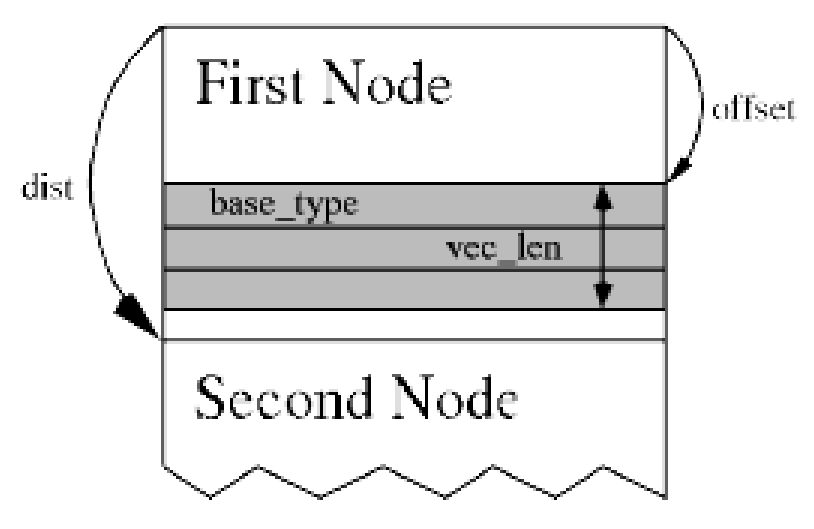
\includegraphics[width=4in]{create_field}
\end{center}
\caption{Creating a Node Field.}
\label{fig:createfield}
\end{figure}

     For example, if you store a 3D force for each node \kw{n}, in an array
indexed by 3*\kw{n}, \kw{vec\_len} is 3, \kw{offset} is 0, and \kw{dist} is
3*8=24.  You can register the node force for update with:

\begin{alltt}
          /* C */
          double *nodeForce;
          ... allocate nodeForce as 3*n_nodes...
          int fid=FEM_Create_Field(FEM_DOUBLE,3,0,24);
 
          ! - Fortran90
          REAL*8 ALLOCATABLE, DIMENTION(:) :: nodeForce
          INTEGER :: fid
          ... allocate nodeForce as 3*n_nodes...
          fid=FEM_Create_Field(FEM_DOUBLE,3,0,24)
\end{alltt}

     If the 3D force is a member \kw{fXYZ} of a structure (in C) or named type
(in Fortran 90) \kw{node\_type}, in an array called \kw{nodes}, you can
register this node force for update with:

\begin{alltt}
          /* C */
          node_type *nodes;
          ...allocate nodes array as n_nodes...
          int fid=FEM_Create_Field(FEM_DOUBLE,3,
              (int)((char *)\&nodes[0].fXYZ-(char *)nodes),
              (int)((char *)\&nodes[1]-(char *)\&nodes[0]) );
 
          ! - Fortran90
          TYPE(node_type), ALLOCATABLE, DIMENTION(:) :: nodes
          INTEGER :: fid
          ...allocate nodes array as n_nodes...
          fid=FEM_Create_Field(FEM_DOUBLE,3,
              offsetof(nodes(1), nodes(1)%fXYZ),
              offsetof(nodes(1), nodes(2)) )
\end{alltt}

     This example uses the Fortran-only helper routine \kw{offsetof}, which
     returns the offset in bytes of memory between its two given
     variables.  The C version uses pointer arithmetic to achieve the
     same result.

\function{void FEM\_Update\_Field(int fid,void *nodes);}
\function{subroutine FEM\_Update\_Field(fid,nodes)}
  \args{integer, intent(in)  :: fid}
  \args{varies, intent(inout) :: nodes}

     Combine a field of all shared nodes with the other chunks.  Sums
     the value of the given field across all chunks that share each
     node.  For the example above, once each chunk has computed the net
     force on each local node, this routine will sum the net force
     across all shared nodes.

     \kw{FEM\_Update\_Field} can only be called from driver, and to be useful,
     must be called from every chunk's driver routine.

     After this routine returns, the given field of each shared node
     will be the same across all processors that share the node.

\function{void FEM\_Read\_Field(int fid,void *nodes,char *fName);}
\function{subroutine FEM\_Read\_Field(fid,nodes,fName)}
  \args{integer, intent(in)  :: fid}
  \args{varies, intent(out) :: nodes}
  \args{character*, intent(in) :: fName}

     Read a field out of the given serial input file.  The serial input
     file is line-oriented ASCII-- each line begins with the global
     node number (which must match the line order in the file),
     followed by the data to be read into the node field.  The
     remainder of each line is unread.  If called from Fortran, the
     first line must be numbered 1; if called from C, the first line
     must be numbered zero.  All fields are separated by white space
     (any number of tabs or spaces).

     For example, if we have called \kw{Create\_Field} to describe 3 doubles,
     the input file could begin with

\begin{alltt}
          1    0.2    0.7    -0.3      First node
          2    0.4    1.12   -17.26    another node
          ...
\end{alltt}

     \kw{FEM\_Read\_Field} must be called from driver at any time, independent
     of other chunks.

\function{void FEM\_Reduce\_Field(int fid,const void *nodes,void *out,int op);}
\function{subroutine FEM\_Reduce\_Field(fid,nodes,outVal,op)}
  \args{integer, intent(in)  :: fid,op}
  \args{varies, intent(in) :: nodes}
  \args{varies, intent(out) :: outVal}

     Combine a field from each node, according to op, across all chunks.
Shared nodes are not double-counted-- only once copy will contribute to the
reduction.  After \kw{Reduce\_Field} returns, all chunks will have identical
values in \kw{outVal,} which must be \kw{vec\_len} copies of \kw{base\_type}.

     May only be called from driver, and to complete, must be called
     from every chunk's driver routine.

     \kw{op} must be one of:

\begin{itemize}
        \item \kw{FEM\_SUM}-- each element of \kw{outVal} will be the sum 
of the corresponding fields of all nodes
        \item \kw{FEM\_MIN}-- each element of \kw{outVal} will be the 
smallest value among the corresponding field of all nodes
        \item \kw{FEM\_MAX}-- each element of \kw{outVal} will be the largest 
value among the corresponding field of all nodes
\end{itemize}

\function{void FEM\_Reduce(int fid,const void *inVal,void *outVal,int op);}
\function{subroutine FEM\_Reduce(fid,inVal,outVal,op)}
  \args{integer, intent(in)  :: fid,op}
  \args{varies, intent(in) :: inVal}
  \args{varies, intent(out) :: outVal}

     Combine a field from each chunk, acoording to \kw{op}, across all chunks.
\kw{Fid} is only used for the \kw{base\_type} and \kw{vec\_len}-- offset and
\kw{dist} are not used.  After this call returns, all chunks will have
identical values in \kw{outVal}.  Op has the same values and meaning as
\kw{FEM\_Reduce\_Field}.

     May only be called from driver, and to complete, must be called
     from every chunk's driver routine.

\subsection{Migration}

The Charm++ runtime framework includes an automated, run-time load balancer,
which will automatically monitor the performance of your parallel program.
If needed, the load balancer can ``migrate'' mesh chunks from heavily-loaded
processors to more lightly-loaded processors, improving the load balance and
speeding up the program.  For this to be useful, pass the \kw{+vpN} argument
with a larger number of chunks \kw{N} than processors-- typically, between 4 and
32 chunks per processor acheive a good trade-off between ability to load
balance and communication overhead.  Because this is somewhat involved, you
may refrain from calling \kw{FEM\_Migrate} and migration will never take place.

The runtime system can automatically move your thread stack to the new
processor, but you must write a PUP function to move any global or
heap-allocated data to the new processor (global data is declared at file scope
or \kw{static} in C and \kw{COMMON} in Fortran77; heap allocated data comes
from C \kw{malloc}, C++ \kw{new}, or Fortran90 \kw{ALLOCATE}).  A PUP
(Pack/UnPack) function performs both packing (converting heap data into a
message) and unpacking (converting a message back into heap data).  All your
global and heap data must be collected into a single block (\kw{struct} in C;
user-defined \kw{TYPE} in Fortran) so the PUP function can access it all.

Your PUP function will be passed a pointer to your heap data block and a
special handle called a ``pupper'', which contains the network message to be
sent.  Your PUP function returns a pointer to your heap data block.  In a PUP
function, you pass all your heap data to routines named \kw{pup\_type}, where
type is either a basic type (such as int, char, float, or double) or an array
type (as before, but with a ``s'' suffix).  Depending on the direction of
packing, the pupper will either read from or write to the values you pass--
normally, you shouldn't even know which.  The only time you need to know the
direction is when you are leaving a processor or just arriving.
Correspondingly, the pupper passed to you may be deleting (indicating that you
are leaving the processor, and should delete your heap storage after packing),
unpacking (indicating you've just arrived on a processor, and should allocate
your heap storage before unpacking), or neither (indicating the system is
merely sizing a buffer, or checkpointing your values).

PUP functions are much easier to write than explain-- a simple C heap block
and the corresponding PUP function is:

\begin{alltt}
     typedef struct {
       int n1;/*Length of first array below*/
       int n2;/*Length of second array below*/
       double *arr1; /*Some doubles, allocated on the heap*/
       int *arr2; /*Some ints, allocated on the heap*/
     } my_block;
 
     my_block *pup_my_block(pup_er p,my_block *m)
     {
       if (pup_isUnpacking(p)) m=malloc(sizeof(my_block));
       pup_int(p,\&m->n1);
       pup_int(p,\&m->n2);
       if (pup_isUnpacking(p)) {
         m->arr1=malloc(m->n1*sizeof(double));
         m->arr2=malloc(m->n2*sizeof(int));
       }
       pup_doubles(p,m->arr1,m->n1);
       pup_ints(p,m->arr2,m->n2);
       if (pup_isDeleting(p)) {
         free(m->arr1);
         free(m->arr2);
         free(m);
       }
       return m;
     }
\end{alltt}

This single PUP function can be used to copy the \kw{my\_block} data into a
message buffer and free the old heap storage (deleting pupper); allocate
storage on the new processor and copy the message data back (unpacking pupper);
or save the heap data for debugging or checkpointing.

A Fortran block TYPE and corresponding PUP routine is as follows:

\begin{alltt}
     MODULE my_block_mod
       TYPE my_block
         INTEGER :: n1,n2x,n2y
         REAL*8, POINTER, DIMENSION(:) :: arr1
         INTEGER, POINTER, DIMENSION(:,:) :: arr2
       END TYPE
     END MODULE
 
     SUBROUTINE pup_my_block(p,m)
       IMPLICIT NONE
       USE my_block_mod
       USE pupmod
       INTEGER :: p
       TYPE(my_block) :: m
       call pup_int(p,m%n1)
       call pup_int(p,m%n2x)
       call pup_int(p,m%n2y)
       IF (pup_isUnpacking(p)) THEN
         ALLOCATE(m%arr1(m%n1))
         ALLOCATE(m%arr2(m%n2x,m%n2y))
       END IF
       call pup_doubles(p,m%arr1,m%n1)
       call pup_ints(p,m%arr2,m%n2x*m%n2y)
       IF (pup_isDeleting(p)) THEN
         DEALLOCATE(m%arr1)
         DEALLOCATE(m%arr2)
       END IF
     END SUBROUTINE
\end{alltt}

\function{int FEM\_Register(void *block, FEM\_PupFn pup\_ud)}
\function{function integer :: FEM\_Register(block,pup\_ud)}
    \args{TYPE(varies), POINTER :: block}
    \args{SUBROUTINE :: pup\_ud}

     Associates the given data block and PUP function.  Returns a block
     ID, which can be passed to \kw{FEM\_Get\_Userdata} later.  Can only be
     called from driver.  For the declarations above, you call
     \kw{FEM\_Register} as:

\begin{alltt}
          /*C/C++ driver() function*/
          my_block *m=malloc(sizeof(my_block));
          int myId=FEM_Register(m,(FEM_PupFn)pup_my_block);
 
          !- Fortran driver subroutine
          use my_block_mod
          interface
            subroutine pup_my_block(p,m)
              use my_block_mod
              INTEGER :: p
              TYPE(my_block) :: m
            end subroutine
          end interface
          TYPE(my_block) :: m
          INTEGER :: myId
          myId=FEM_Register(m,pup_my_block)
\end{alltt}

     Note that Fortran blocks must be allocated on the stack in driver;
     while C/C++ blocks may be allocated on the heap.

\function{void FEM\_Migrate()}
\function{subroutine FEM\_Migrate()}

     Informs the load balancing system that you are ready to be
     migrated, if needed.  If the system decides to migrate you, the
     PUP function passed to \kw{FEM\_Register} will be called with a sizing
     pupper, then a packing, deleting pupper.  Your stack (and pupped
     data) will then be sent to the destination machine, where your PUP
     function will be called with an unpacking pupper.  \kw{FEM\_Migrate}
     will then return, whereupon you should call \kw{FEM\_Get\_Userdata} to
     get your unpacked data block.  Can only be called from driver.

\function{void *FEM\_Get\_Userdata(int n)}

     Return your unpacked userdata after migration-- that is, the
     return value of the unpacking call to your PUP function.  Takes
     the userdata ID returned by \kw{FEM\_Register}.  Can be called from
     driver at any time.

     Since Fortran blocks are always allocated on the stack, the system
     migrates them to the same location on the new processor, so no
     \kw{Get\_Userdata} call is needed from Fortran.
\input{index}
\end{document}
